\chapter{\iftoggle{german}{Konzept}{Concept}}\label{ch:concept}

In this section we discuss about the dataset and design choice,\todo and the rationale behind reducing the domain gap.

\section{Pix3D: A large-scale benchmark}\label{s:Pix3D}
In ~\cite{pix3d}, a large-scale benchmark for 2D-3D alignment was introduced.
The raw images from web search engines were collected and labelled keypoints were used to align the 2D images with the corresponding 3D shapes.
The 3D models are extension from IKEA dataset~\cite{Lim2013ParsingIO}, which is a collection of high-quality IKEA furniture.
The dataset also provides with masks and keypoints for the object under observation.
For adding more images to the IKEA dataset, the authors of ~\cite{pix3d} conducted manual web search on Google, Bing, and Baidu, using Ikea model name as keywords.
to get around 104,220 images which were further filtered by removing irrelevant images with the help of Amazon Mechanical Turk (AMT) workers.
After this manual experiment the total images in Pix3D, only 14,600 images were selected for the 219 Ikea models.
For our experiment on synthetic to real dataset, we chose to select only furniture classes from Pix3D, leaving out "misc and tools" classes, which were significantly less to begin with.


\subsection{Disadvantages of Pix3D}

The distribution of models in pix3d is as shown in ~\ref{fig:pix3d_histogram}.
As we can see, the dataset distribution is uneven across classes and more than 50\% of classes have less than 1000 images.

Though Pix3D set a benchmark for 2D-3D alignment, here are few disadvantages of using this real dataset.
\begin{enumerate}
    \item For Deep Learning approches, we need large-scale data and 14,600 might not be sufficient.
    \item The orientation of object is not randomised.
    \item The dataset does not provide 2.5D information (i.e. depth and normal) which can be crucial for 3D learning.
\end{enumerate}

\begin{figure}[!ht]
    \centering
    \subfloat[][]{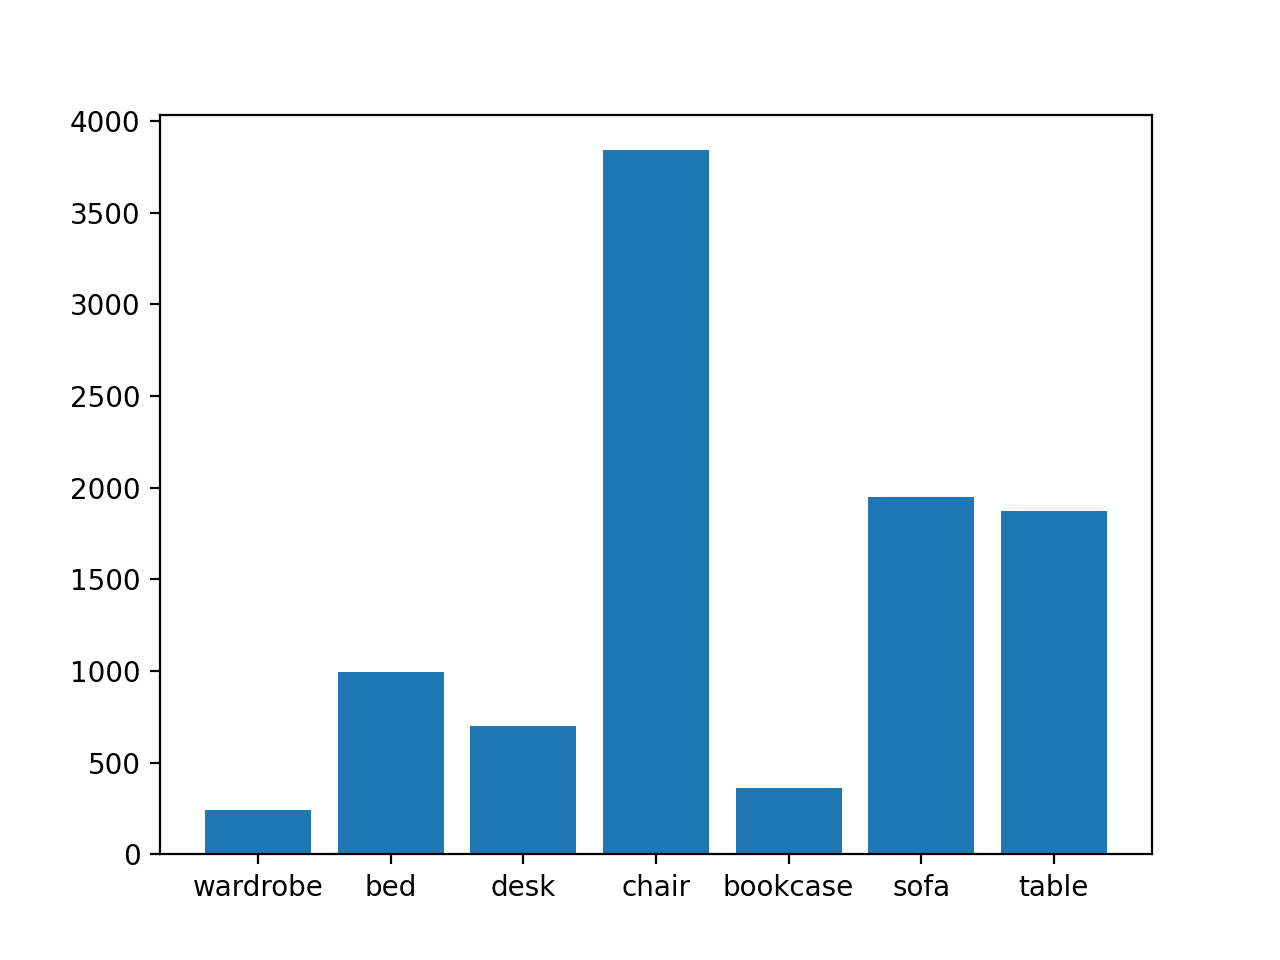
\includegraphics[width=.45\textwidth,height=6cm]{/Users/apple/OVGU/Thesis/code/3dReconstruction/report/images/pix3d/pix3d_histogram}}\quad
    \subfloat[][]{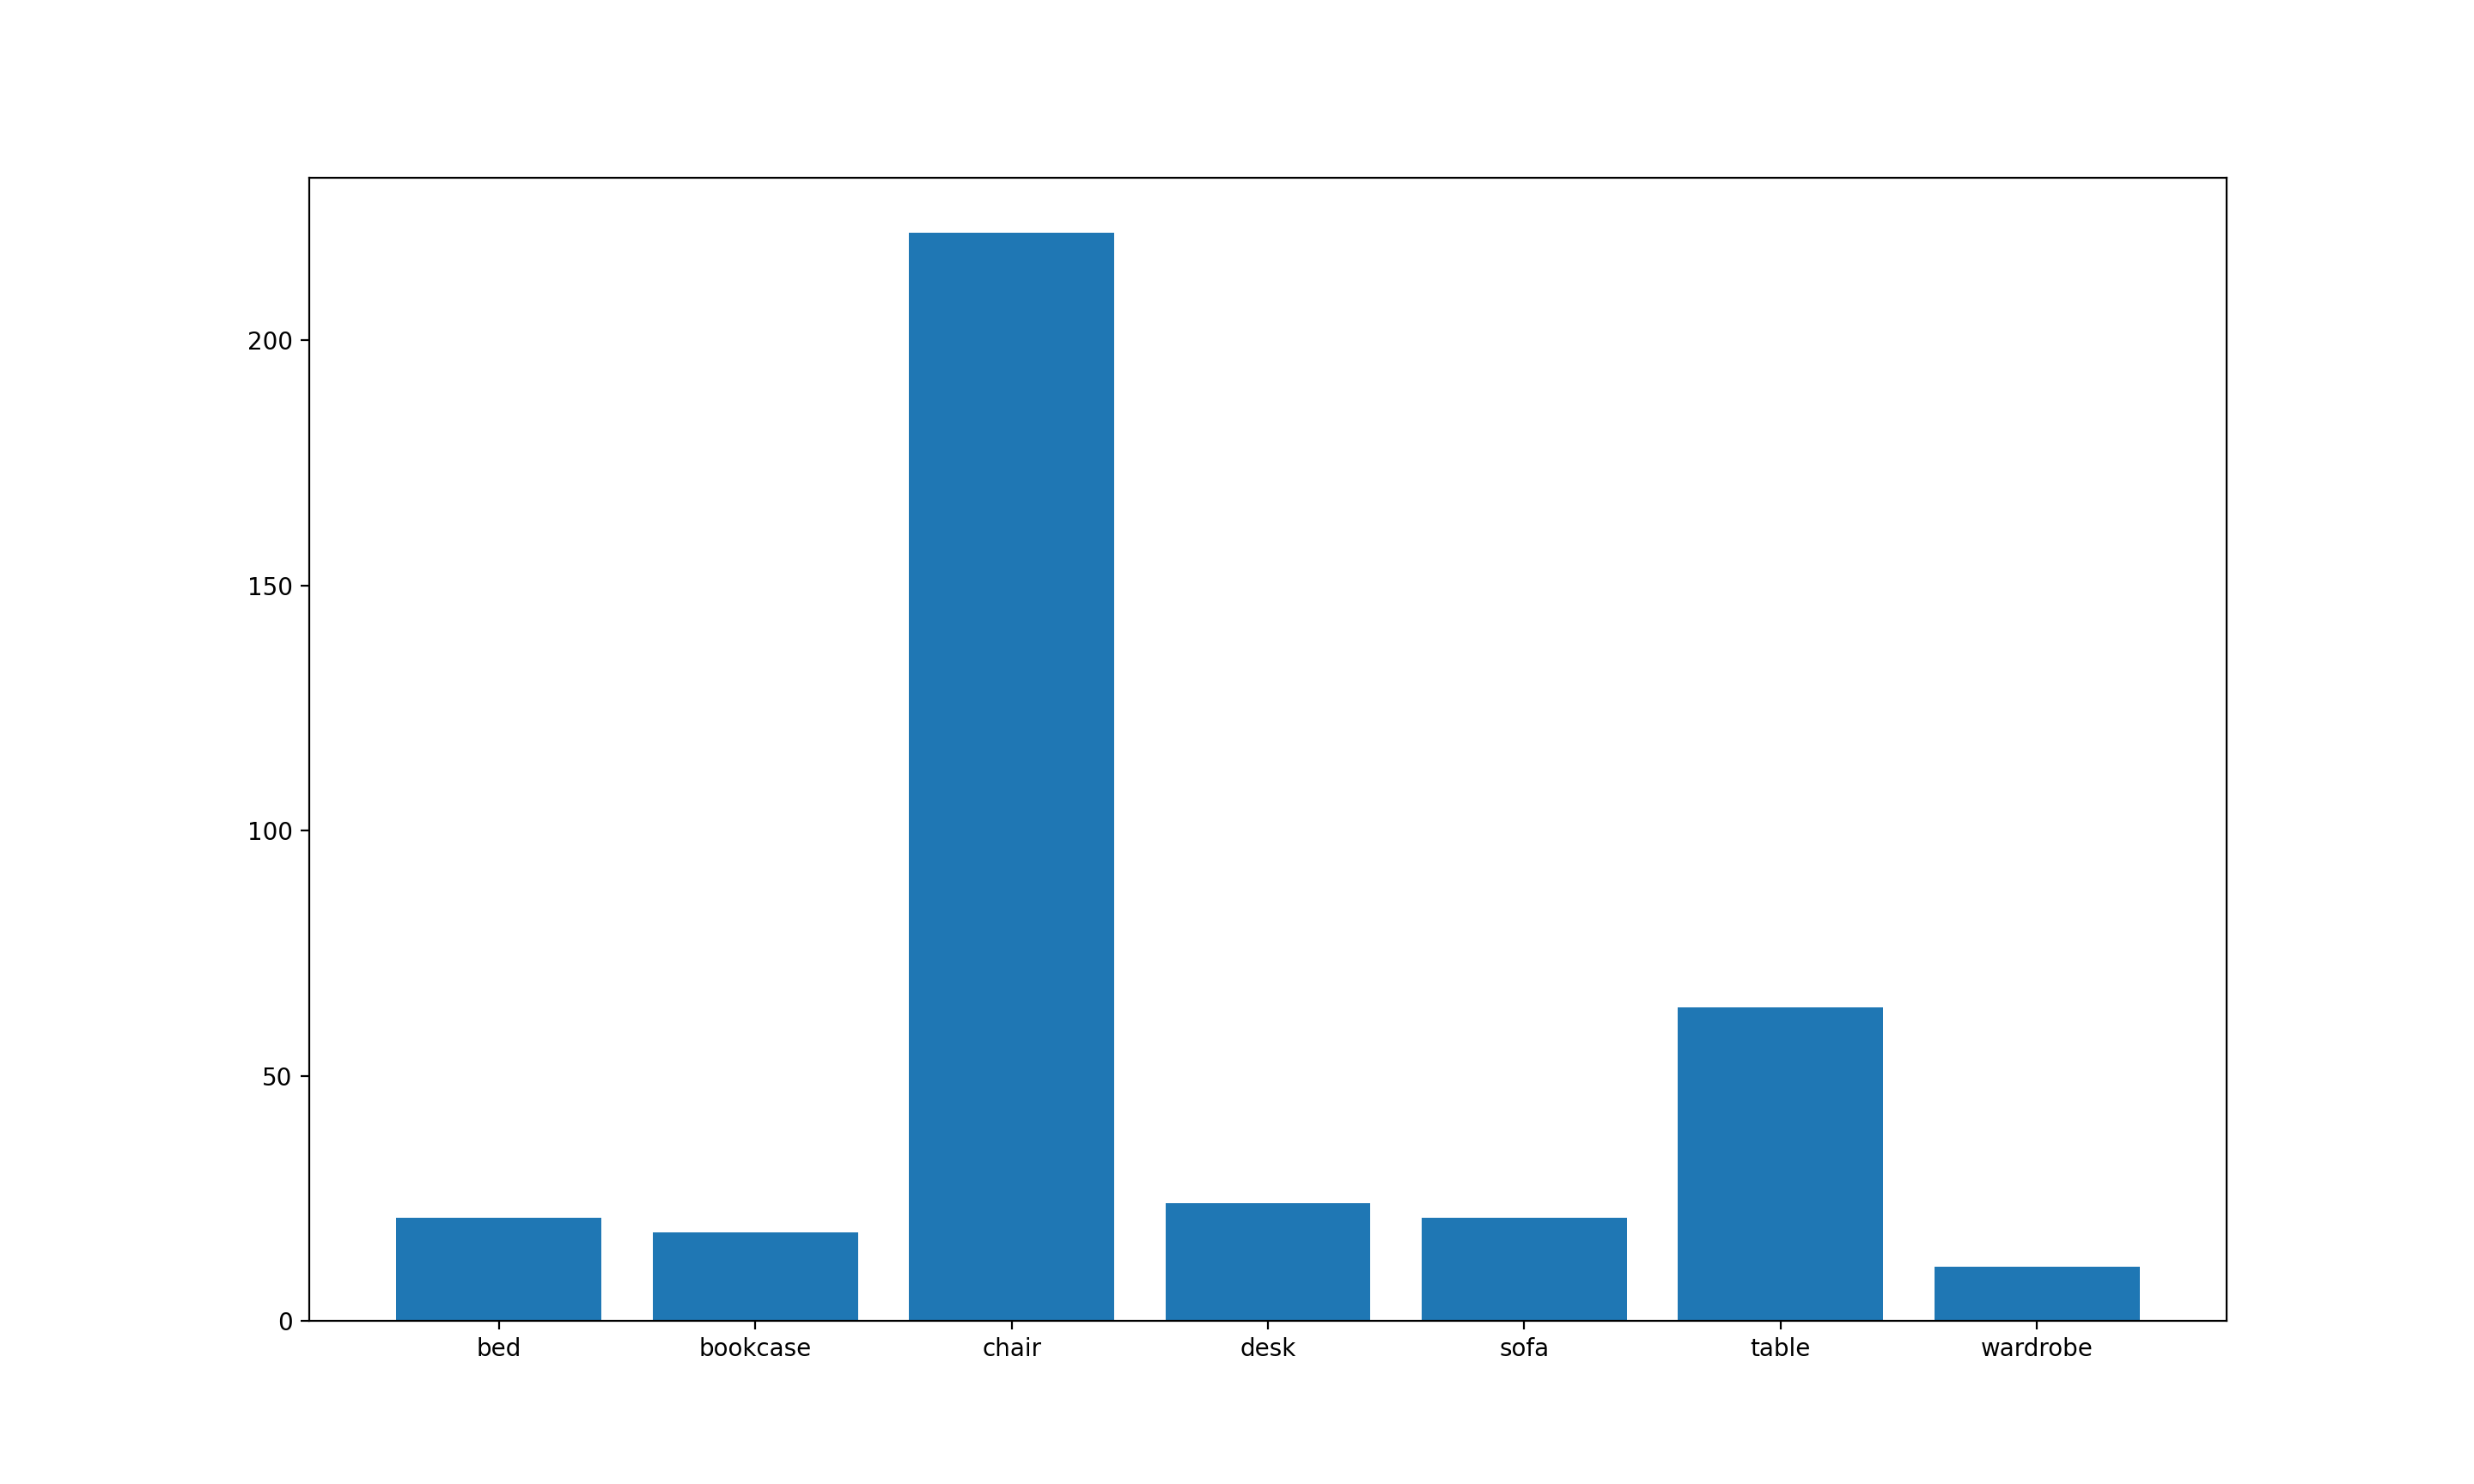
\includegraphics[width=.45\textwidth,height=6cm]{/Users/apple/OVGU/Thesis/code/3dReconstruction/report/images/pix3d/pix3d_models_histogram}}\\
    \caption{Distribution of pix3D~\cite{pix3d} images(left), unique models(right)}
    \label{fig:pix3d_histogram}
\end{figure}

\subsection{Why Pix3D?}
    Pix3D is a collection of indoor scenes with complex background, varying light conditions with shadows, reflective surfaces and even varying occlusion levels
    .Each image comprises of collection of objects in the scene, but only one object from the catagory is annotated. It is a perfect example of having limited real world data.
    And since 3D models are available for each furniture,a synthetic data can be generated in abundance from those models.

\begin{figure}[!ht]
    \centering
    \subfloat[][]{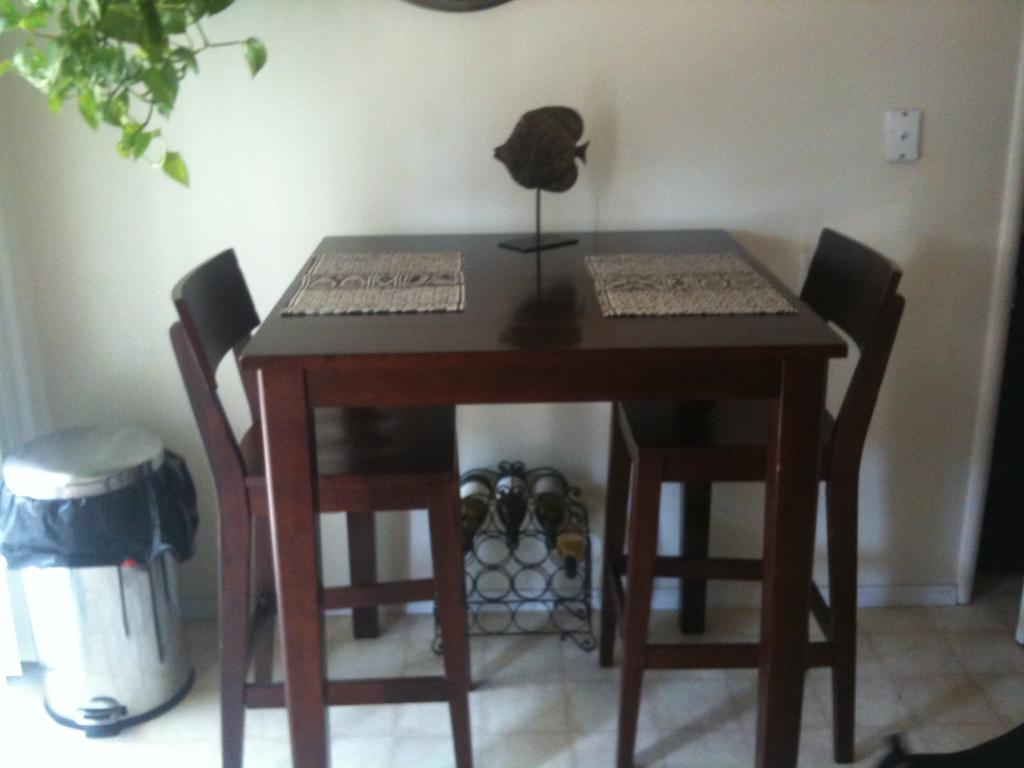
\includegraphics[width=.4\textwidth]{/Users/apple/OVGU/Thesis/code/3dReconstruction/report/images/pix3d/pix3d_5}}\quad
    \subfloat[][]{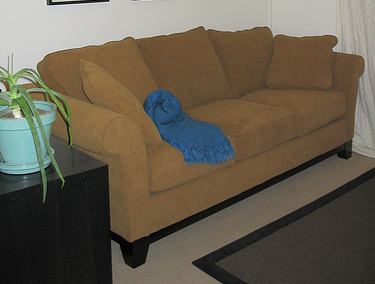
\includegraphics[width=.4\textwidth]{/Users/apple/OVGU/Thesis/code/3dReconstruction/report/images/pix3d/pix3d_2}}\\
    \subfloat[][]{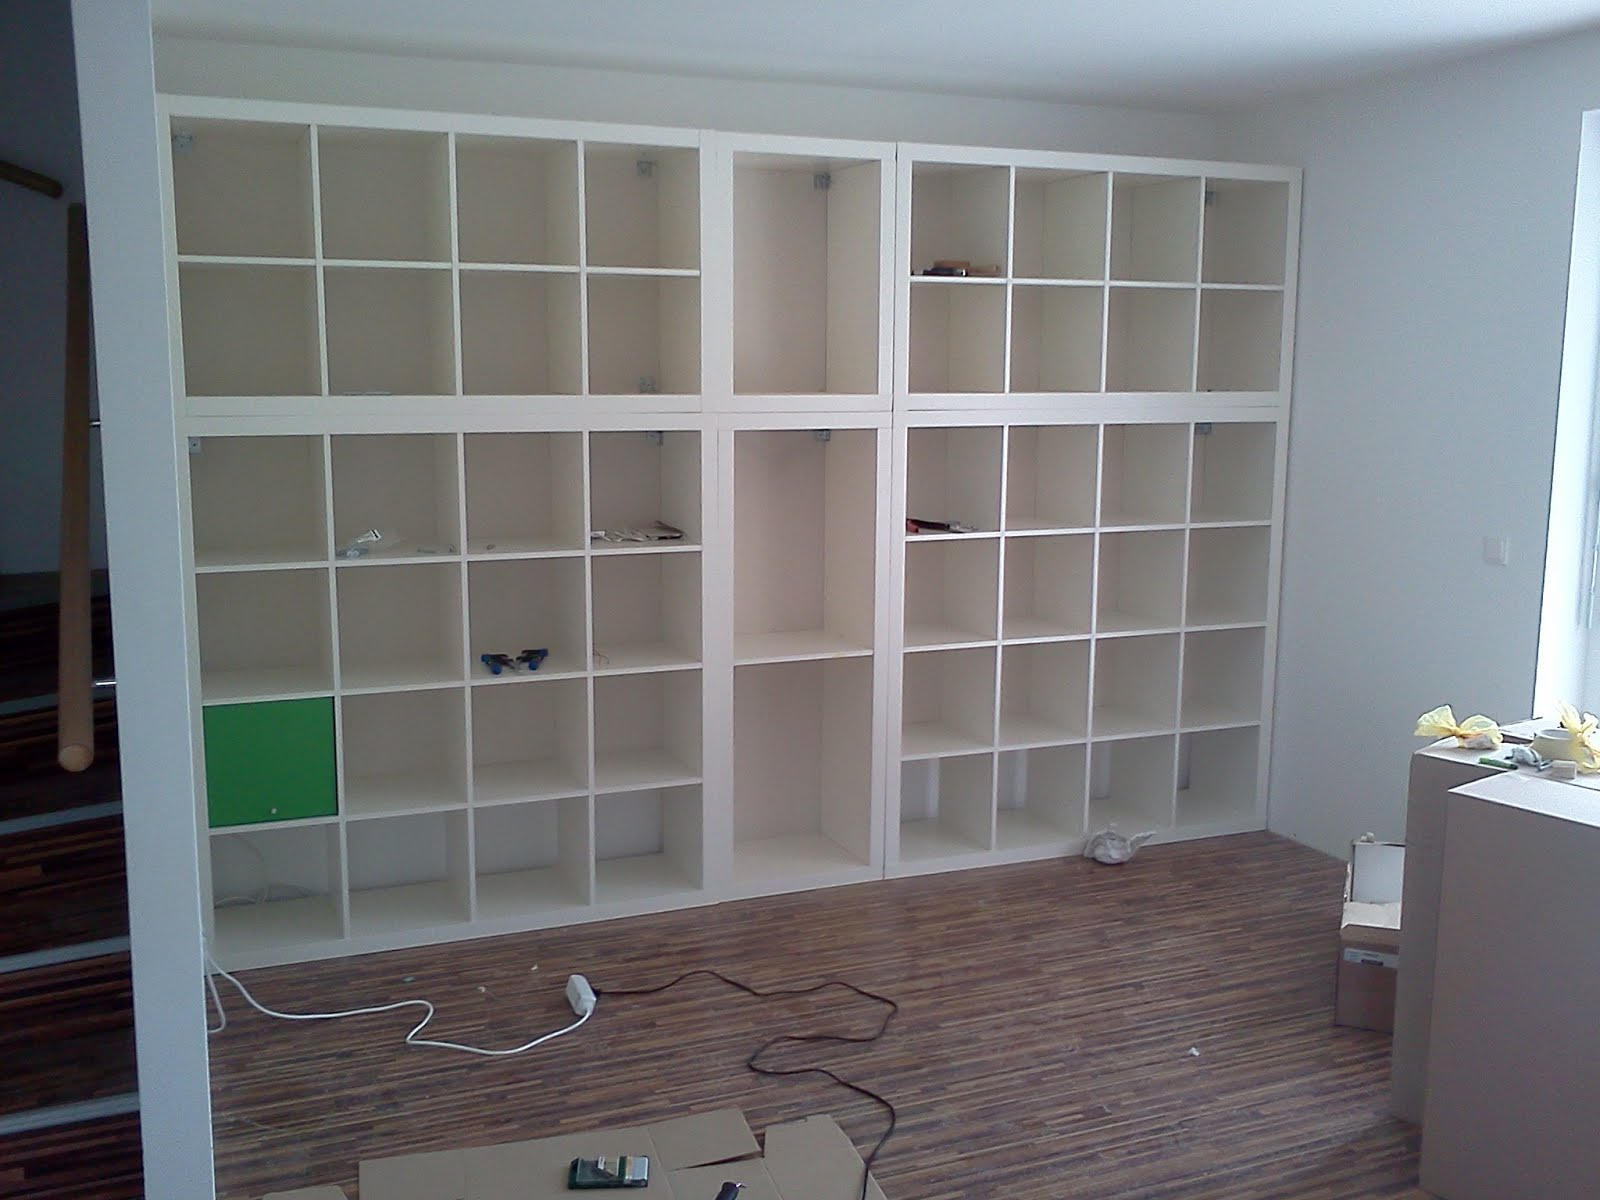
\includegraphics[width=.4\textwidth]{/Users/apple/OVGU/Thesis/code/3dReconstruction/report/images/pix3d/pix3d_6}}\quad
    \subfloat[][]{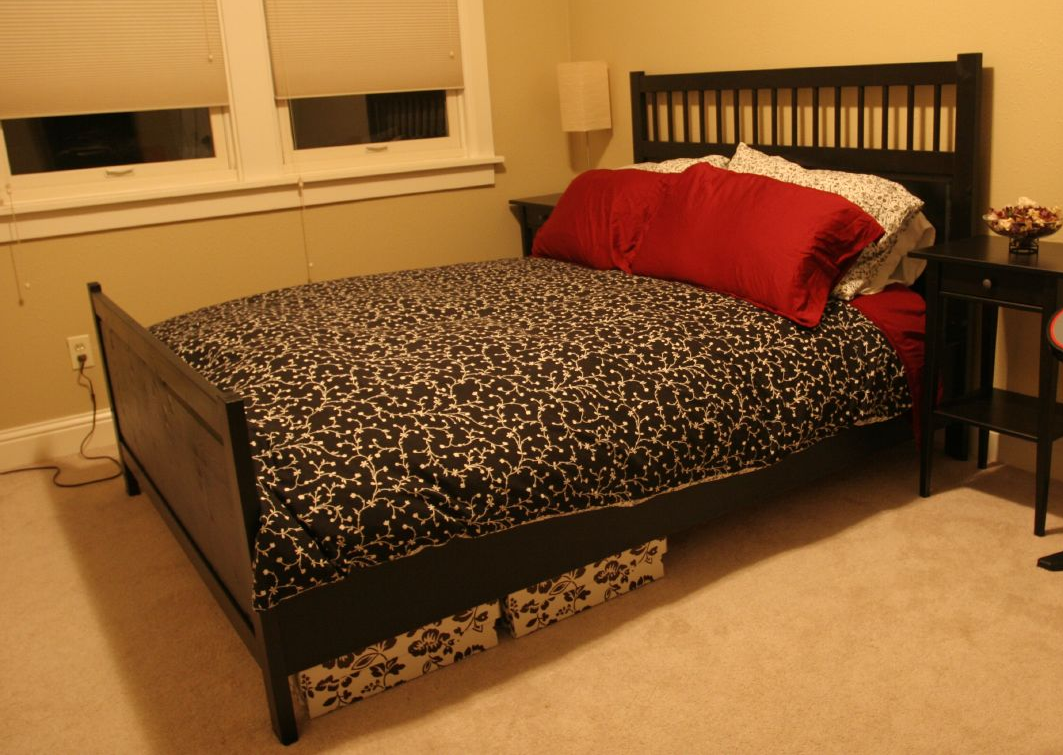
\includegraphics[width=.4\textwidth]{/Users/apple/OVGU/Thesis/code/3dReconstruction/report/images/pix3d/pix3d_4}}
    \caption{Sample RGB images from pix3D}
    \label{fig:Pix3D samples}
\end{figure}

\section{Role of SceneNet}\label{ss:SceneNet}
    SceneNet ~\cite{McCormac:etal:ICCV2017} is a large collection photorealistic indoor scene trajectories.
    The dataset provides with images and videos of indoor scene which can be used for tasks like SLAM, semantic and instance segmentation,
object detection and further enhanced for other vision problems like optical flow depth and pose estimation ~\cite{McCormac:etal:ICCV2017}).
They use ShapeNet~\cite{chang2015shapenet} models to occupy 57 indoor scenes which gives the scene unlimited configurations.
Unfortunately there is no mapping from scene to 3D model for tasks like 3D reconstructions.
In our approach, we utilize the scene provided by SceneNet as layout for our indoor scenes. This includes initial shapenet models with furniture placement.
We then replace the class under observation with a corresponding model from Pix3D.

\section{Unity based pipeline}\label{ss:Unity Pipeline}
Unity game engine is used for creating the synthetic dataset.
The reasons for selecting Unity as our platform for the application are:
\begin{enumerate}
    \item Cross-platform game engine and hence can be used on an Operating system.
    \item The basic version is available for free.
    \item Provides all the necessary tools to create an ersatz environment with well maintained documentation.
    \item An active developer community.
\item \end{enumerate}

There is no official comparison between Unreal Engine and Unity engine to have a deciding factor.
The selection of unity engine was purely individual choice and ease of use.
But both these game engines have ability to create realistic looking scenes which can be used for synthetic dataset generation.
With Unity game engine, the available scenes from scenenet and 3D models from pix3d can be imported to form an ersatz environment.
Further domain randomisation can be applied to create a dataset of photorealistic images and 2.5D data like normal, depthmaps, masks.

\subsection{Domain Randomisation with Unity Engine}\label{ss:Domain Randomisation with unity engine}
In this section we discuss what kind of domain randomisation is applied for the dataset creation.
\subsubsection{Scenes from scenenet}
As discussed in section ~\ref{ss:SceneNet}, SceneNet provides wide variety of indoor scenes which includes bedrooms, bathroom, living room, kitchen and office.
For our case, we did not consider bathroom as the class under observations are furnitures and we rarely have any furnitures in the bathroom.
For the rest of the scenes we have a pre-determined setup given by scenenet. We use 25 scenes in total as basic rooms for our target object to be place.
And with further randomisation we feel this should be sufficient to check if unity can produce a useful dataset.

\subsubsection{Camera Viewpoints}
The position and orientation of camera gives us the most randomisation in this setup.
The minimum and maximum distance can be chosen by the user for the camera to be places from the target object.
A random point can be selected in this range as the position for the camera.
As for the orientation of the camera, we can make the camera to always look at the target object, irrespiective of the position.
With this, we acheived different background for target object, and the target object itself appears to be in different position and orientation.

\subsubsection{Lighting and shadows}
Lighting plays an important role in photorealism. If the lighting is not setup correctly the synthetic dataset will never seem to be photorealistic.
Unity offers wide variety of lighting like global light which acts like the sunlight, and various indoor lighting systems.
Ideally we should make the luminous objects like lamps, chandlier, bulbs etc be the source of light for indoor scenes, but we observed that the room does not lit up uniformly which makes in less photorealistic.
Hence we use some pre-determined lighting settings which will be further discussed in implementation section ~\ref{s:3D-Scene framework}.

\subsubsection{Randomised textures}
SceneNet ~\cite{McCormac:etal:ICCV2017} also provides with textures for different categories in the scene.
We then further increase the texture database by adding few more textures from ambientCG.com, which provide license for free.
We randomly allocate textures to each object making sure that each category has same texture to make the scene more uniform.

\subsubsection{Replacing target objects}
To further randomise the scene, the category of target objects in the scene are replaced by the object under observation.
When there are more than one object of same category we randomise the selection of which object is to be replaced which further randomises the captured data.
The scale of the target object is made to match the scale of the category object in the scene in the least dimension.
For example if the length of the length of the category object in the scene is the least amonth length,width and height, then the target object is scaled to match this length.
This makes the target object blend in with the scene.

\section{S2R:3D-FREE, a Pix3D based sythetic dataset}

S2R:3D-FREE dataset, which stands for Synth2Real: 3-Dimensional Furniture Reconstruction from Ersatz Environment, is a combination of SceneNet and Pix3D dataset.
We utilize the avalaibilty of 3D models of rooms and furntitures from these 2 dataset to create an ersatz environment using Unity as our framework.
We randomise the indoor scenes from SceneNet ~\cite{McCormac:etal:ICCV2017} along with textures provided by them with some additional complex textures.
The other option would have been to use the shapenet as the target model, but in this case we would not be having a real dataset to compare to.
Ideally a model trained on shapenet should also perform well with a real dataset like pix3d, but we decided to have a synthetic dataset based on pix3d itself for better comparison.


\section{3D reconstruction pipeline}
Now that we discussed on how the dataset will be created, we move to the deep learning aspect of this thesis.
\subsection{Pix2Vox and Pix2Vox++}
The architecture of pix2vox ~\cite{Xie_2019} as in ~\ref{fig:pix2vox architecture}.
The network is comprised of 4 modules: Encoder, Decoder, Merger and Refiner.
Merger plays significant part when it comes to mult-view reconstruction of 3d objects.
But we focus on single-view 3d reconstruction and hence merger will not influence the output significantly.
As Encoder, pix2vox has utilised VGG16 network ~\cite{simonyan2015deep} pre-trained on ImageNet ~\cite{Deng2009ImageNetAL}.
Decoder is an expansive network which converts 2D embeddings to 3D voxel grid.
Refiner is an auto-encoder which takes the 3D output from the merger and produces more refined final output.
A second paper based on pix2vox was titled Pix2Vox++ ~\cite{Xie_2020}.
The extended work replaces VGG encoder ~\cite{simonyan2015deep} with ResNet ~\cite{He2016DeepRL}.

\subsubsection{Why Pix2Vox?}
Pix2Vox has been used as baseline by most of the research oriented to 3D reconstruction.
This network is one of the few networks to be tested on pix3d dataset.
According to the survey conducted by ~\cite{Han2021ImageBased3O}, performance of pix2vox ~\cite{Xie_2019}
has been noted to be significantly higher when compared to previous work \todo{cite other papers} as shown in \ref{fig:survey on 3d reconstruction}.
While this comparison was made on 3d reconstuction of shapenet dataset, since pix3d was not available at the time when previous work were published.
From our survey, only CoReNet ~\cite{popov2020corenet} had a slight gain in performance compared to pix2vox.
When trained on shapenet and tested with pix3d, CoReNet gave a result of 29.7\% IoU while Pix2Vox gave a result of 28.8\% IoU and Pix2Vox++ a result of 29.2\% IoU.
Since the difference in the performance was not statistically significant we decided to stick with the baseline model itself.
Another reason for selecting pix2vox model is that the backbone of the architecture is pre-trained with ImageNet and
hence the embeddings generated from this encoder can help in visualising the domain space of both Pix3D (real images) and S2R:3DFREE(synthetic images).
As mentioned above, for pix2vox++ the Resnet is the backbone encoder which has 25\% lesser parameters and 5\% lesser inference time compared to VGG.
In addition, the author even proved that Pix2vox++ performs 1.5\% better than pix2vox.
Furthermore, the focus of this thesis is not to check which is the best model to reconstruct the model, but to check if game engines can produce photorealistic images usable for 3d reconstruction.
Hence the selection of the model was not of utmost importance.
But since the 2 architecture are relatable, it would be interesting to compare the results for 3d Reconstuction task.
\begin{figure}
    \centering
    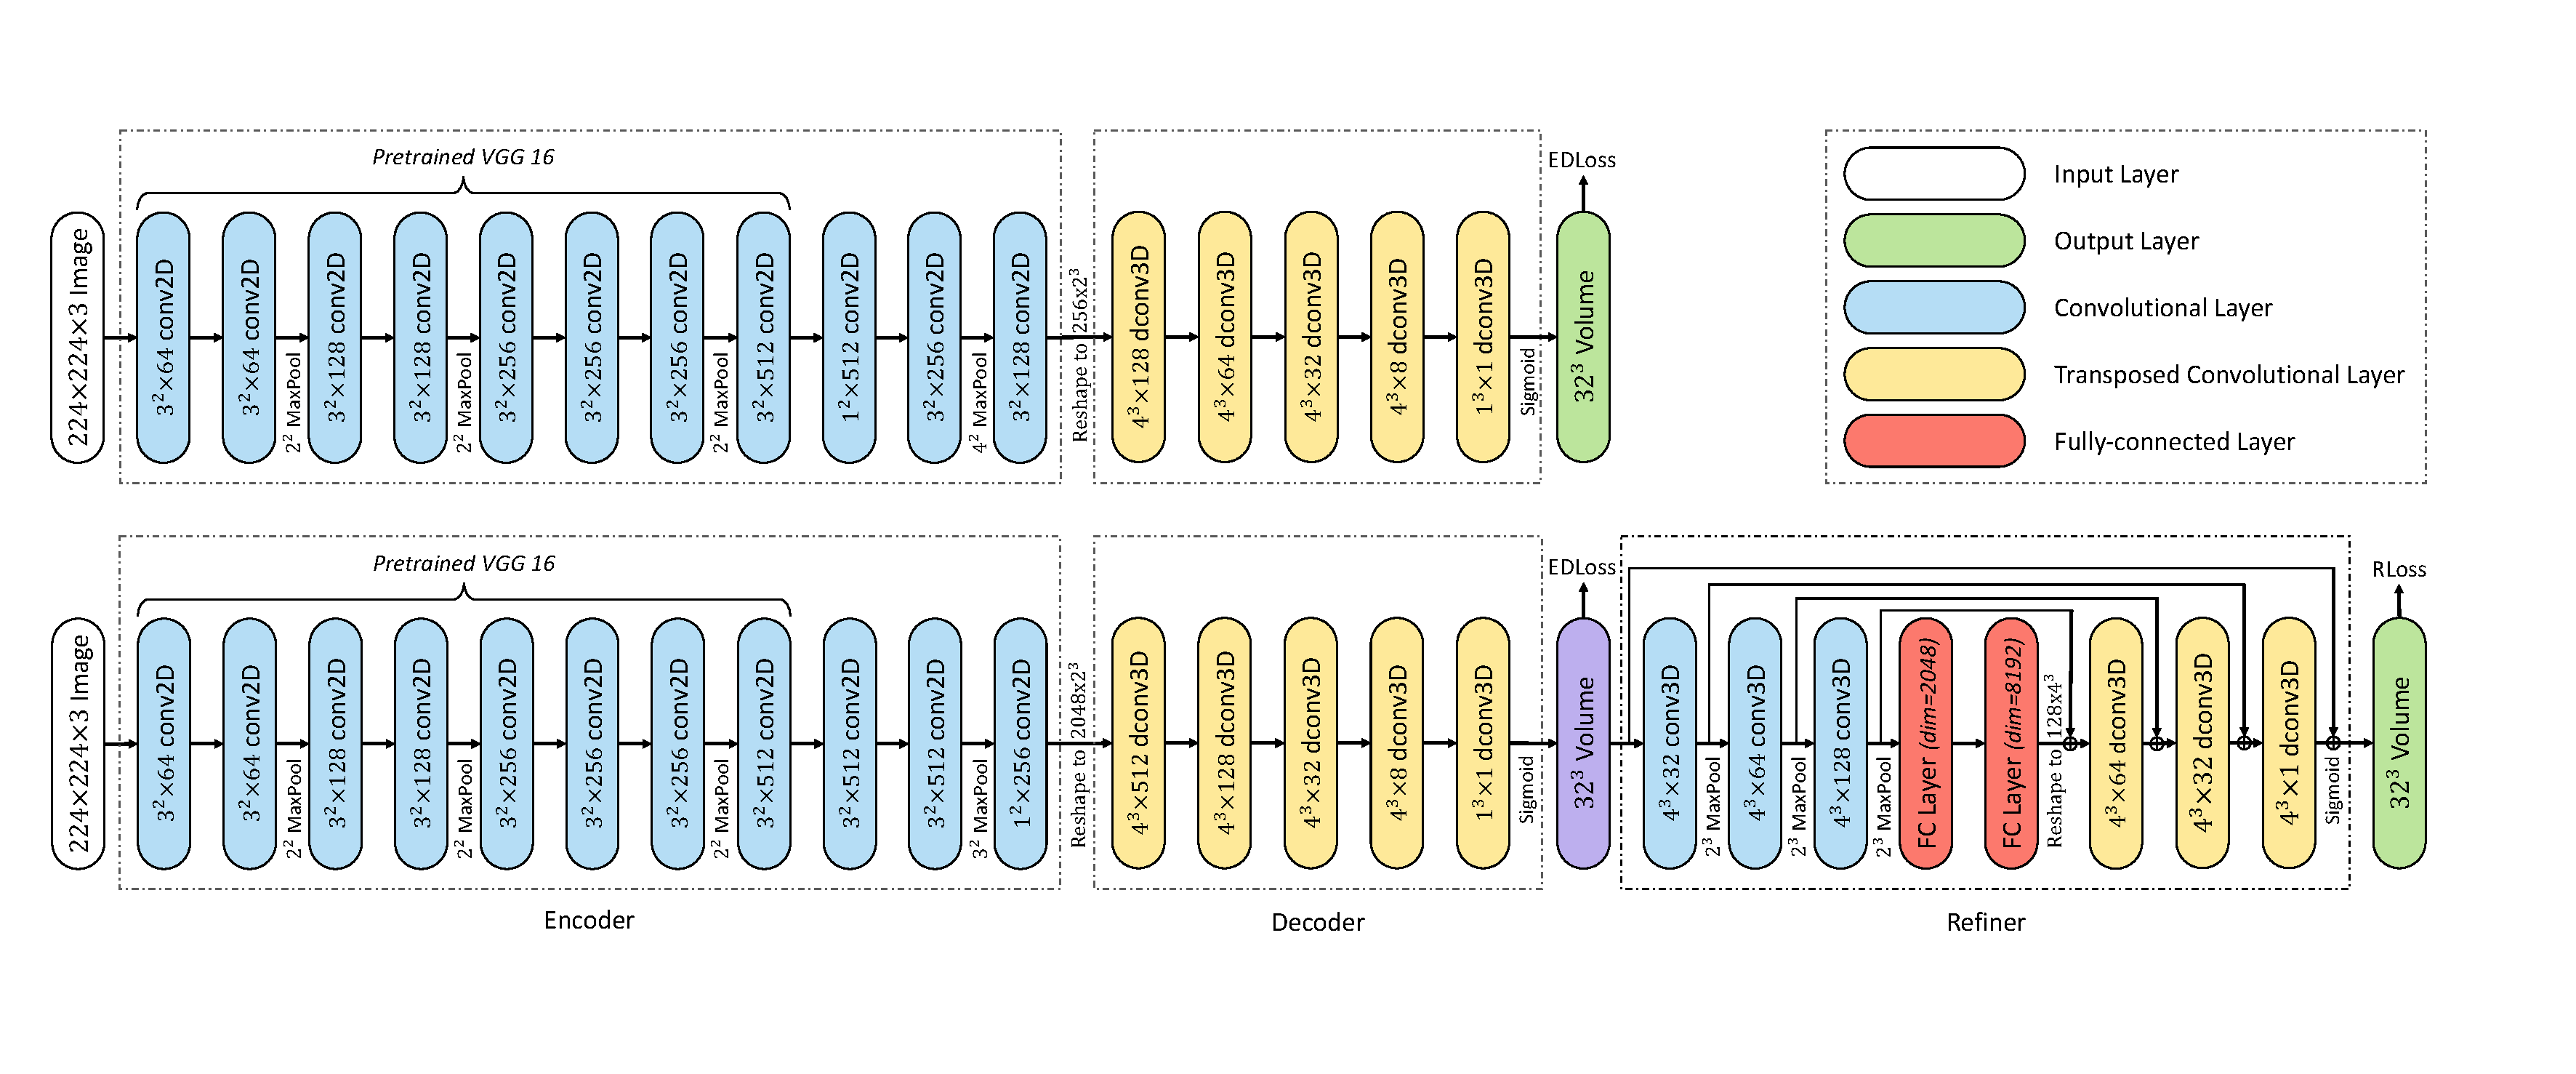
\includegraphics[width=1\textwidth]{/Users/apple/OVGU/Thesis/code/3dReconstruction/report/images/concept/pix2vox}
    \caption{Network architecture for pix2vox~\cite{Xie_2019}}
    \label{fig:pix2vox architecture}
\end{figure}

\begin{figure}
    \centering
    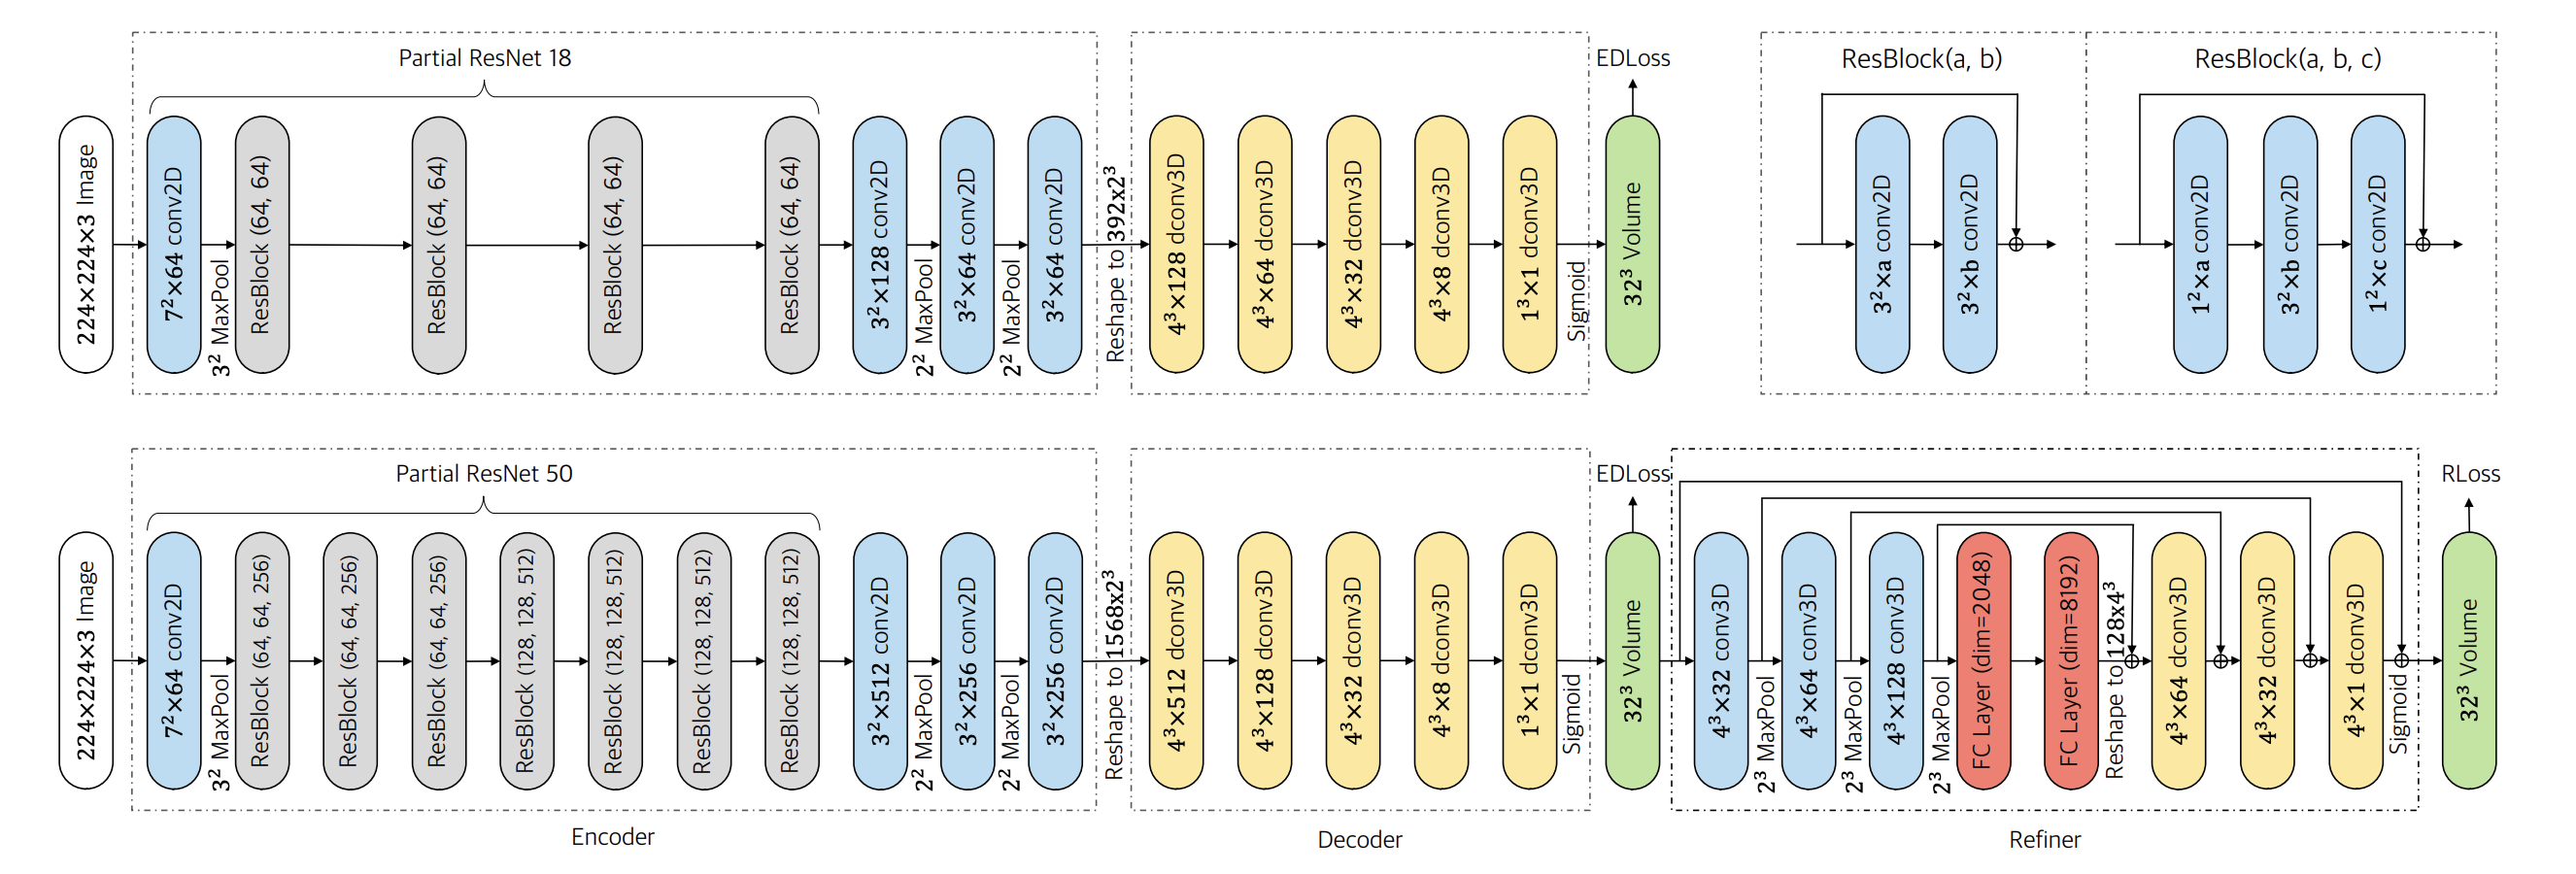
\includegraphics[width=1\textwidth]{/Users/apple/OVGU/Thesis/code/3dReconstruction/report/images/concept/pix2voxpp}
    \caption{Network architecture for pix2vox++~\cite{Xie_2020}}
    \label{fig:pix2voxpp architecture}
\end{figure}

\begin{figure}
    \centering
    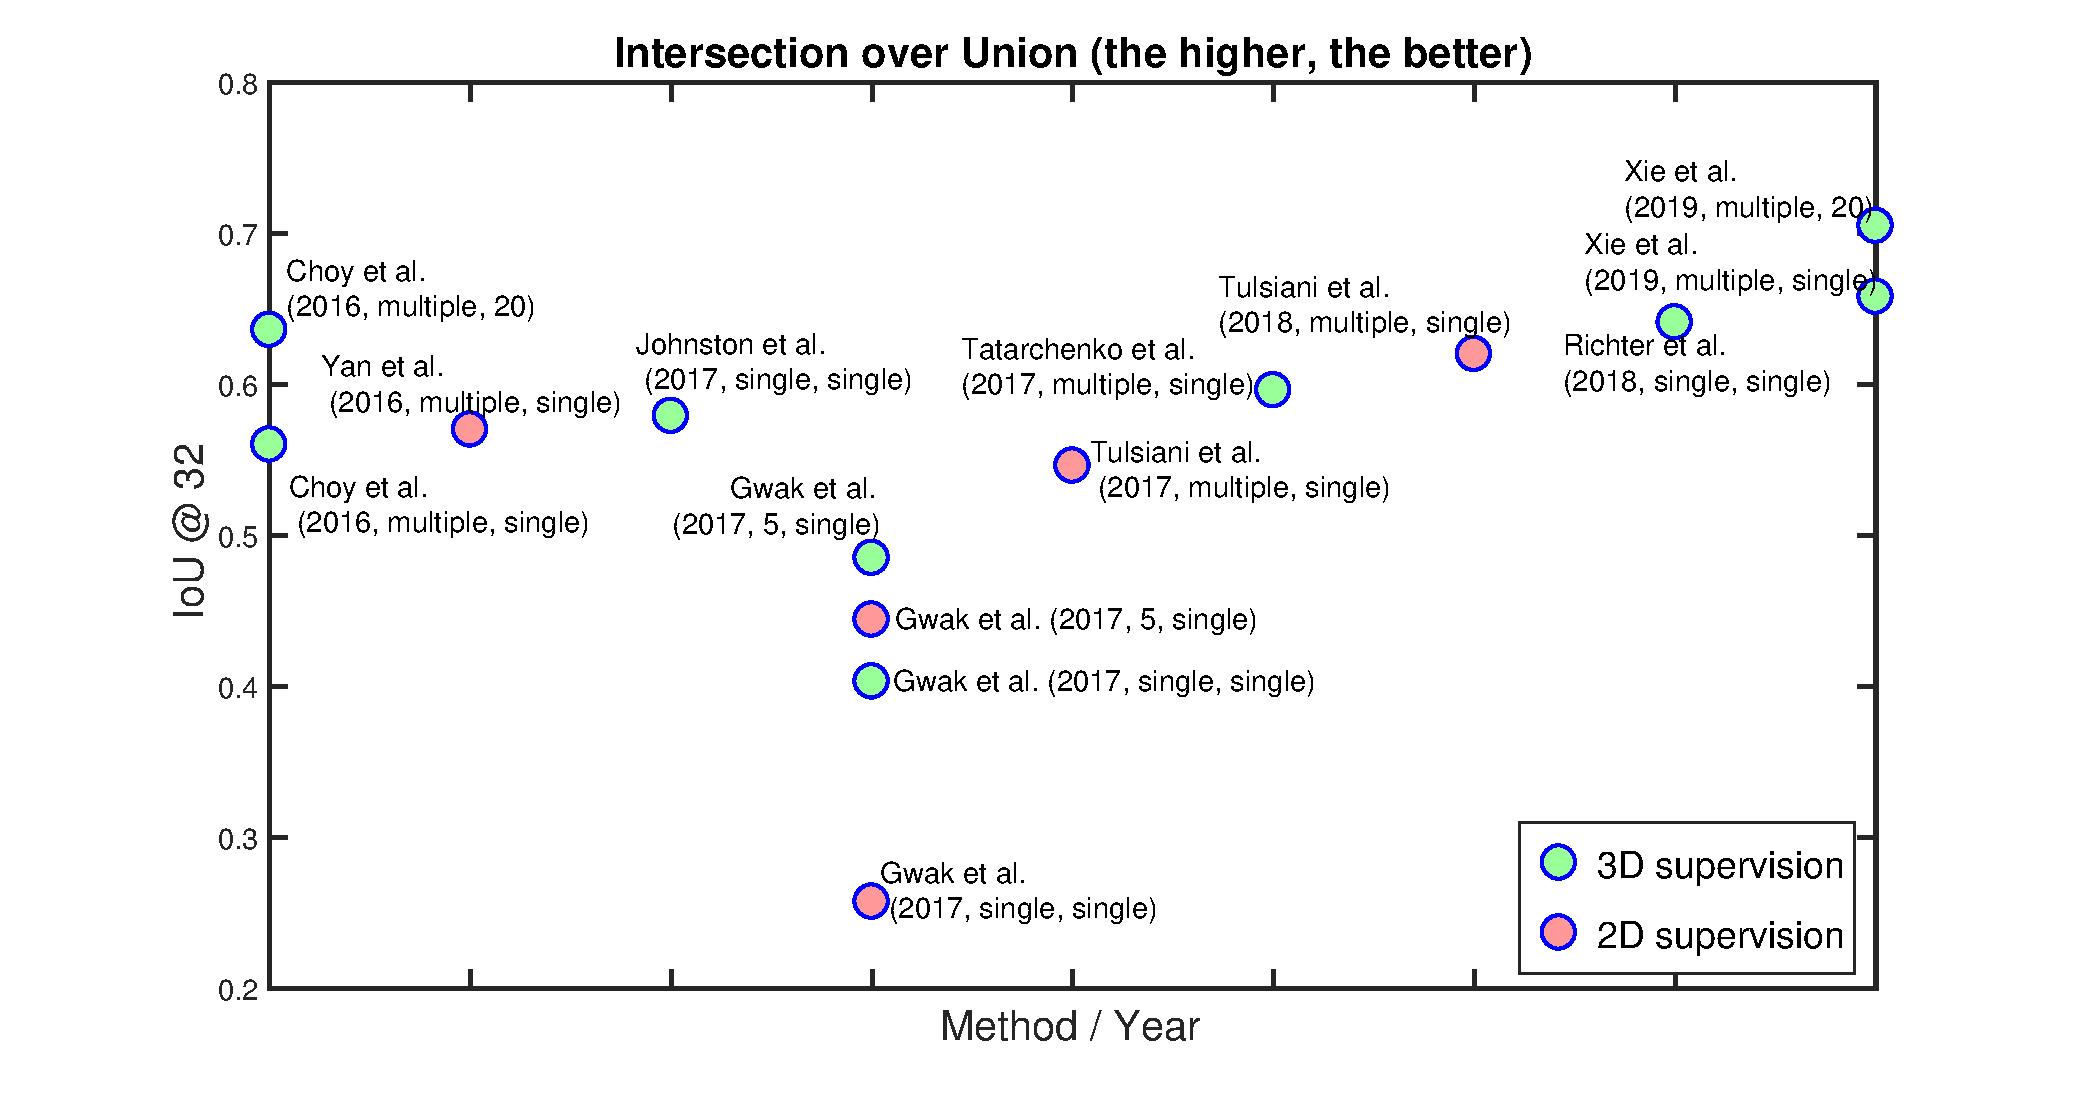
\includegraphics[width=1\textwidth]{/Users/apple/OVGU/Thesis/code/3dReconstruction/report/images/concept/survey}
    \caption{A survey conducted by ~\cite{Han2021ImageBased3O}, proves that Pix2Vox is considerably a good 3D reconstruction model.
    \todo{replace this figure with better one}}
    \label{fig:survey on 3d reconstruction}
\end{figure}

\section{Domain adaptation with Gan \todo{if we decide to go with this approach}}

\section{Training}
\todo re-write
\cite{seib2020mixing} proved mixed training with synthetic and real dataset improves the performance. They used 40\% mixing ratio

\cite{2018LearningIC} used mixing ratios for classification task for each of the minibatches and observed 5-13\% improvement in performance.